\section{Experiments}
\noindent{\textbf{Data}} To fairly evaluate the effect of cycle regularization, we use the datasets released by AtlasNet and Pixel2Mesh respectively. Their model sets are both subsets of ShapeNet \cite{shapenetdata} and they both used the rendered images from \cite{3DR2N2} \mdf{with sizes of $224 \times 224$}. However, the absolute sizes and positions of the models and the sampled points as ground truth are not processed in the same way in these two datasets, which makes it unreasonable to compare them all together. Therefore we evaluate the effect of our regularization technique with these two networks separately with their own released data.

\noindent{\textbf{Training}}
Unless specifically explained, the network models shown in this paper are trained as follows. The parameters for image encoders and forward 3D decoders $\theta_f$ are initialized with parameters released by AtlasNet \cite{atlasnet} and Pixel2Mesh \cite{pixel2mesh} respectively. The parameters for inverse decoders $\theta_g$ are randomly initialized. We use the ADAM \cite{adam} optimizer with the same learning rate as in the original codes of AtlasNet and Pixel2Mesh respectively. We use $\lambda=0.25$ as an empirical choice for the weight of our cycle regularization term.

\noindent{\textbf{Evaluation Criteria}}
In order to quantitatively evaluate the issue of self-intersection and self-overlap, we count the percentage of self-intersected triangles (``SI") over the total number of triangles. For this evaluation, we provide our code in the supplemental material which calculates the ``SI" for an input mesh.  
We also use the value of Chamfer distance (``CD") as the original AtlasNet and Pixel2Mesh to evaluate how well the generated mesh approximates the ground truth shape. For the evaluation of Chamfer distance we used the codes that are already implemented by AtlasNet \cite{atlasnet} and Pixel2Mesh \cite{pixel2mesh}.

\noindent{\textbf{Mesh Generation and Visualization}} Since we are addressing an issue regarding the quality of generated mesh, any post-processing used in AtlasNet \cite{atlasnet} is not used in our \mdf{experiments}. All the triangulations are directly transfered from the predefined surface. We do not divide the triangles to get denser vertices either. The meshes from AtlasNet all have 2500 vertices and about 4k faces. The meshes from Pixel2Mesh all have 2466 vertices and 4928 faces.

To better expose the issue we are addressing in this paper, we render the generated mesh in MeshLab and use the ``gooch.gdp" in the software as our shader. In such mode, triangles are rendered golden outside and bluish inside. The golden region and bluish region interlacing at surface evidently indicates the self-intersected surfaces.

\subsection{Visualization of Deformation Process}
\label{subsec:deform}
\begin{figure}
	\centering
	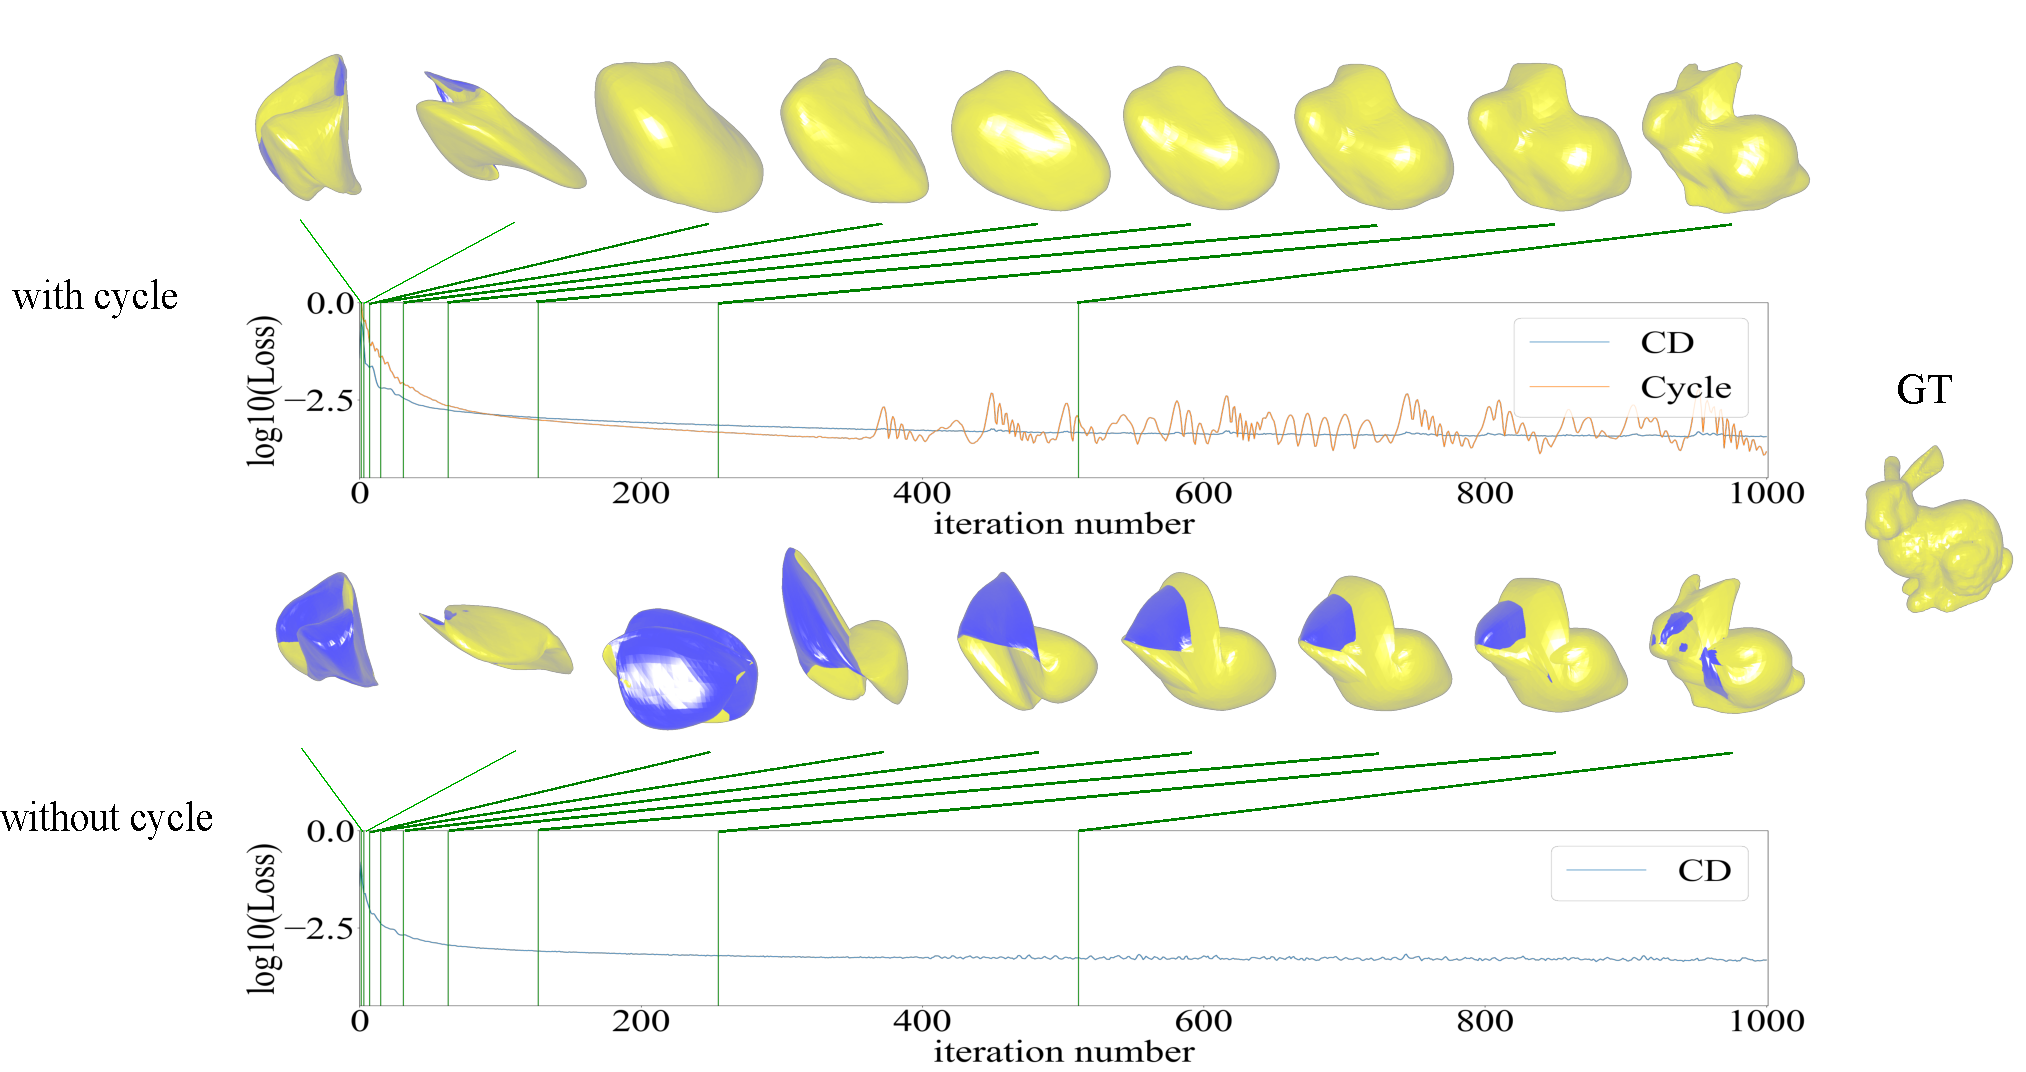
\includegraphics[width=\linewidth]{img/opt/opt2}
	\caption{\mdf{Convergence of optimization. When optimized with our cycle regularization term, the term takes effect after only a few iterations. It does not only keep the mapping injective during optimization but also corrects the self-intersection from the initialization. When optimized without cycle regularization term, the surface usually converges to a surface with self-intersection.}}
	\label{fig:opt}
\end{figure}
\begin{wrapfigure}{r}{0.48\textwidth}
	\begin{center}
		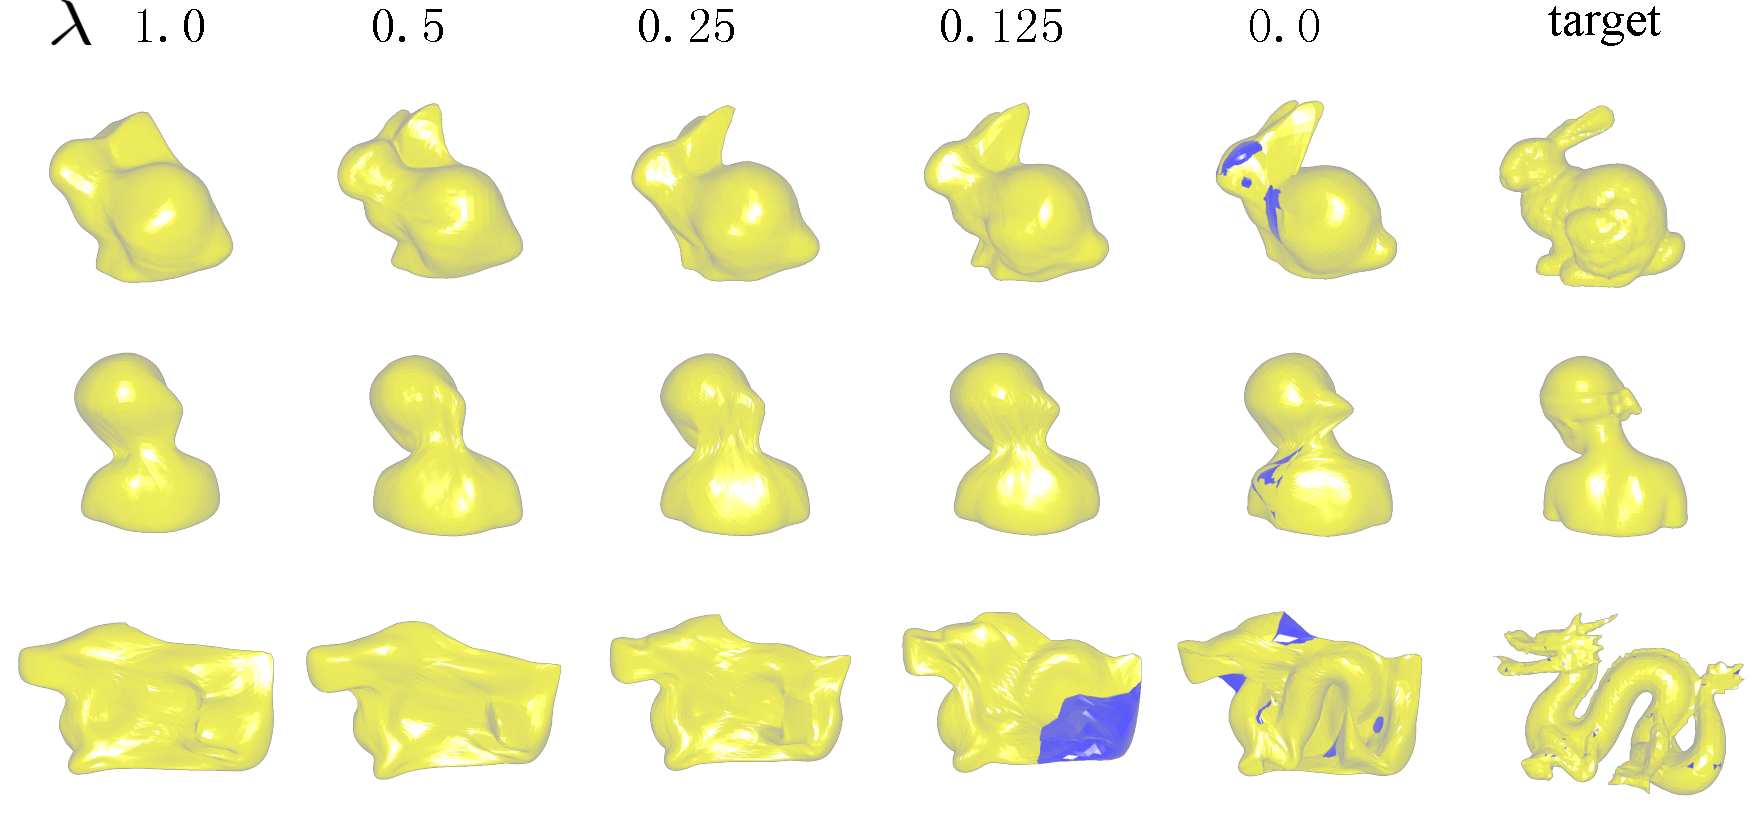
\includegraphics[width=0.48\textwidth]{img/opt/lambda}
	\end{center}
	\caption{Deformation results with different $\lambda$.}
	\label{fig:lambda}
\end{wrapfigure}
\begin{figure}
	\centering
	\includegraphics[width=\linewidth]{revision/img/torus/torus}
	\caption{Exploration into higher genus: The columns of ``init"  are intial output shapes. The columns of ``with cycle" or ``without cycle" are final output shapes optimized with or without cycle regularization term. Under each final output shape, we report its chamdfer distance(CD) to ground truth, cycle regularization loss (Cycle, if used) at the end of iteration and the percentage of self-intersection(SI). }
	\label{fig:torus}
\end{figure}
In this subsection, we visualize the deformation process, providing a more intuitive view into the effect of our cycle regularization term. Being free of self-intersection is a rather geometric prior for surface mesh than a semantic one. Therefore, we do not involve any semantic networks and show the effect of our proposed technique in a pure shape deforming manner (different from the training neural networks) in this experiment. In other words, we optimize the same objective function as in Eq.~(\ref{equ:atlascycle}), but do not use semantic networks (neither ResNet-18 \cite{resnet} nor PointNet \cite{pointnet}) to generate the latent shape representation $\mathbf{s}$. We treat $\mathbf{s}$ as \mdf{a free variable}. We use the same MLP for $f$ and $g$ as in Eq.~(\ref{equ:atlascycle}), but we only deform the generated shape to approach a specific groundtruth shape. We initialize the parameters $\theta_f,\theta_g,\mathbf{s}$ randomly with standard normal distribution and sample $X$ from sphere surface. We use ADAM \cite{adam} as the optimizer with $0.001$ as learning rate. \mdf{We set maximum iteration number to $1024$ for all experiments in this subsection. As shown in Figure~\ref{fig:opt}, $1024$ iteration is usually more than enough for the optimization to converge.} Under such setting, we are deforming a randomly initialized shape (probably start with self-intersection) to approach a specific groundtruth shape. As the case shown in Figure~\ref{fig:opt}, our cycle regularization term takes effect after only a few iterations. It not only keeps the mapping injective in following iterations but also corrects the self-intersections from the random initialization.

We experiment on different $\lambda$ controlling the contribution of the cycle regularization term in the entire objective function. As shown in Figure~\ref{fig:lambda}, visually speaking, when $\lambda=0.25$, the deformed shape is able to approximate more details than a larger value (i.e. $\lambda=0.5,1.0$), and it is also sufficient to enforce the injective mapping.  Therefore we use $\lambda=0.25$ as an empirical choice in following experiments. However, finer tuning for specific networks is possible.

\mdf{We also explore into cases with higher genus by manually choose torus as source surface. Though this is not a viable approach to enable nerual network to generate shapes with complex topology, it allows us to observe the effect of our cycle regularization in the case of genus-1. As shown in Figure~\ref{fig:torus}, our observation can be concluded as follows: With torus as source surface, cycle regularization can still significantly reduce self-intersection (looking at ``SI") and preventing the collapse of the hole. As shown in the cases of ``okay" and``love", the outputs are wildly self-intersected and the hole from the source toruses both collapsed. However, the optimization is more easily to get stuck at a local minimum where the remaining self-intersected triangles tends to concentrate and form two knots. With sphere as source surface, though the outputs are not able to express the hole in the groundtruth, they are less likely to get stuck at a local minimum with self-intersection.  
}

\subsection{Cycle Regularization in AtlasNet and Pixel2Mesh}
\begin{figure}
	\centering
	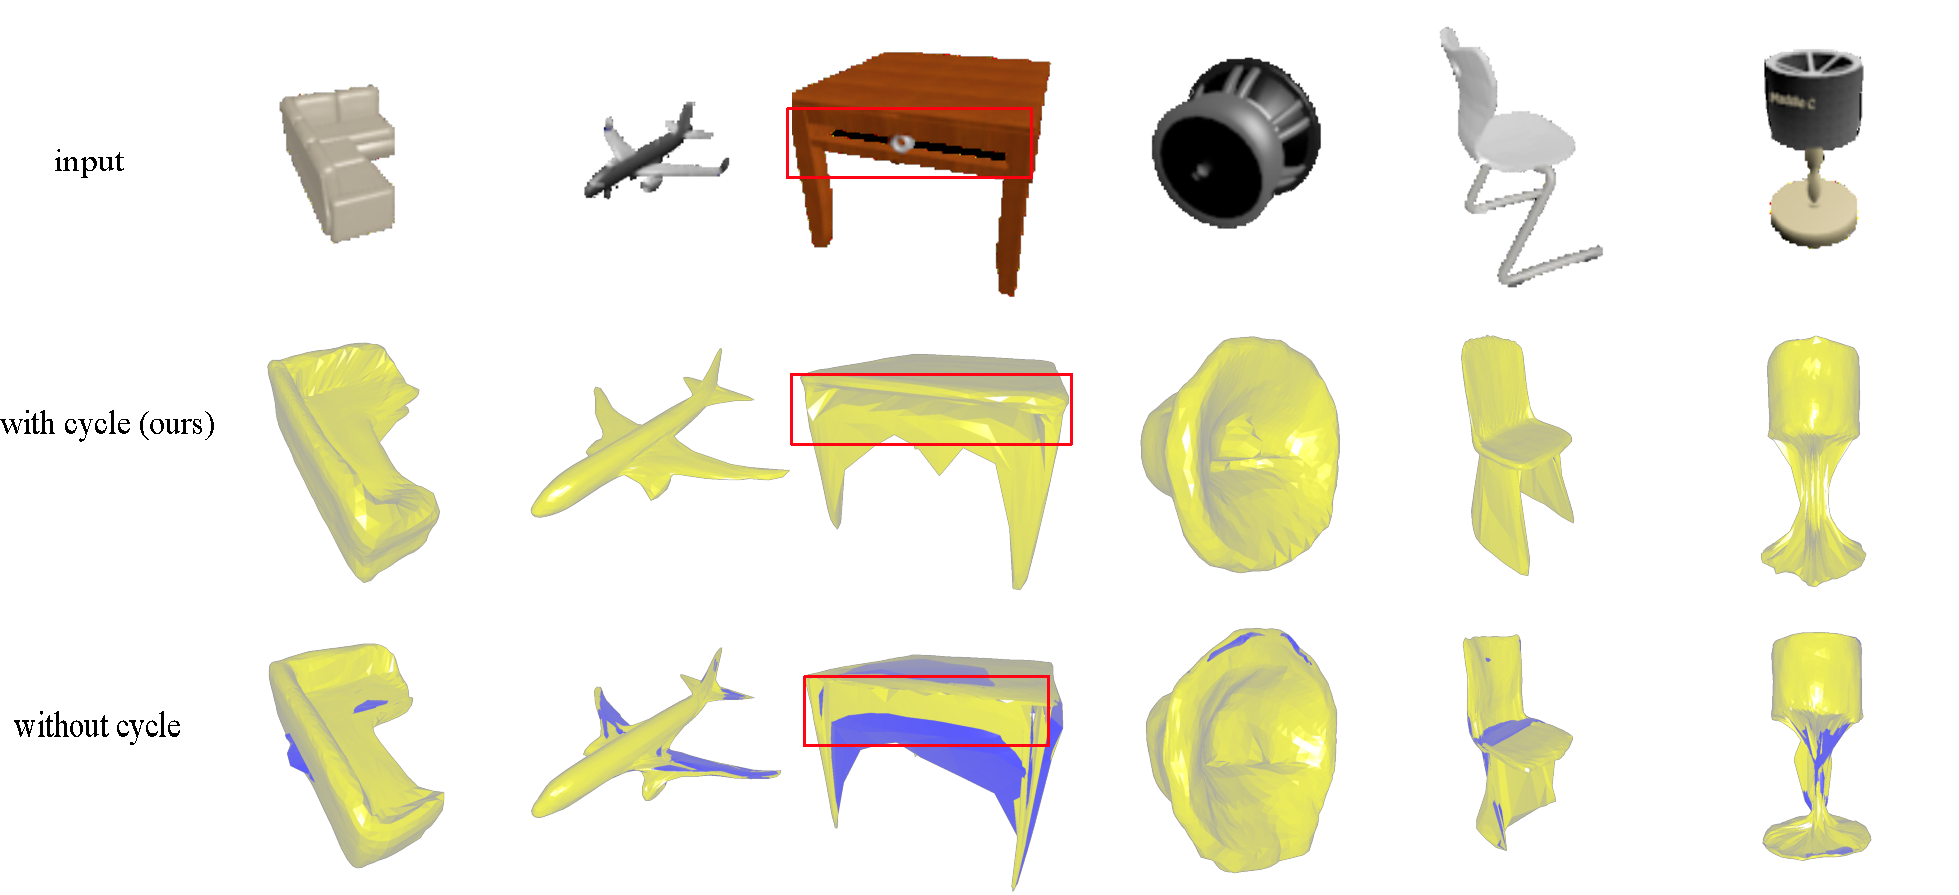
\includegraphics[width=\linewidth]{img/atlas/svr}
	\caption{Cycle regularization on AtlasNet. All the visualized cases here are selected from the test set of AtlasNet. Some meshes' view direction are manually adjusted to better expose the differences. The red rectangles highlight a case where more details are preserved than the original network because injectivity is enforced with our cycle regularization.}
	\label{fig:svr}
\end{figure}
\begin{figure}
	\centering
	\includegraphics[width=\linewidth]{img/p2m/final}
	\caption{Cycle regularization on Pixel2Mesh. All the visualized cases here are selected from the test set of Pixel2Mesh. Some meshes' view direction are manually adjusted to better expose the differences.}
	\label{fig:p2m}
\end{figure}
\begin{figure}
	\centering
	\includegraphics[width=\textwidth]{img/p2m/3level}
	\caption{Visualization of the effect of our cycle regularization in the coarse-to-fine framework of Pixel2Mesh. The green rectangle shows a close-up view of a subtle self-intersection.}
	\label{fig:3level}
\end{figure}
In this subsection, we conduct experiments to evaluate our cycle regularization along with two latest networks, AtlasNet \cite{atlasnet} and Pixel2Mesh \cite{pixel2mesh}. We report the quantitative evaluation for AtlasNet and Pixel2Mesh in Table~\ref{tab:atlas} and Table~\ref{tab:p2m} respectively. We show visual examples for AtlasNet and Pixel2Mesh in Figure~\ref{fig:svr} and Figure~\ref{fig:p2m} respectively. It can be seen that after applying our cycle regularization, the percentage of self-intersected triangles are significantly reduced, while the generated shapes remain comparable to the shapes generated by original networks.

More specifically, in Table~\ref{tab:atlas}, we show evaluation on AtlasNet in two tasks, auto-encoding (AE) and single view reconstruction (SVR). The auto-encoding task reconstructs a complete 3D mesh from a point set (encoded by PointNet\cite{pointnet} to generate shape representation feature $\mathbf{s}$) which constains relatively more complete information about the 3D shape. The single view reconstruction task takes a single view image (encoded by ResNet-18 \cite{resnet} to generate $\mathbf{s}$) as input and also reconstructs a complete 3D mesh. Therefore, it is easier to reach lower Chamfer distance (0.0017) in auto-encoding and it is harder for further improvement.  In single view reconstruction, there are cases, as highlighted by red rectangles in Figure~\ref{fig:svr}, that preventing self-intersections provides extra prior knowledge for the network to learn to generate more details for the generated shape. We believe this is perhaps why our performance in ``CD"  are slightly worse than original AtlasNet in auto-encoding (0.0019 vs. 0.0017) but slightly better than original AtlasNet in single view reconstruction (0.0050 vs. 0.0052). Nevertheless, both the ``SI" criteria in Table~\ref{tab:atlas} and the visual examples in Figure~\ref{fig:svr} supports that the proposed cycle regularization can effectively reduce self-intersections in AtlasNet. Averagely, the percentage of self-intersected faces in our generated meshes decreases about two orders of magnitude comparing to meshes generated by original networks.

In Table~\ref{tab:p2m}, we show evaluation on Pixel2Mesh. For Pixel2Mesh our model is slightly worse than original Pixel2Mesh in terms of Chamfer distance. We believe this is because we have not yet properly investigated how our cycle regularization term interferes with other loss terms in Pixel2Mesh. We should be able to tune a better model in future. However, we believe both the overall performance in Table~\ref{tab:p2m} and the visual examples in Figure~\ref{fig:p2m} are already evidently enough to support the main idea in this paper that the proposed cycle regularization can significantly reduce self-intersection in the generated meshes for Pixel2Mesh. In Figure~\ref{fig:3level}, we provide more visual examples proving that the proposed cycle regularization takes effect in all three levels in Pixel2Mesh's coarse-to-fine framework.

\begin{table}
	\caption{Evaluation on AtlasNet trained with(\textbf{ours}) and without cycle regularization. Chamfer distance(CD) ($10^3$ times at left) and percentage of self-intersected(SI) faces (at right) are reported. ``AE" stands for the shape auto-encoding task, and ``SVR" stands for single view reconstruction task. Sphere means that the models are using sphere as predefined surface to sample points from. The mean is data-wise as it is implemented in the evaluation code of AtlasNet.}
	\label{tab:atlas}
	\centering
	\begin{tabular}{|c|rc|rc|rc|rc|}
		\hline 
		~&\multicolumn{4}{c|}{AE-sphere}&\multicolumn{4}{c|}{SVR-sphere}\\
		\cline{2-9}
		~& \multicolumn{2}{c|}{AtlasNet} & \multicolumn{2}{c|}{Ours} & \multicolumn{2}{c|}{AtlasNet} & \multicolumn{2}{c|}{Ours} \\
		\hline
		cellphone&1.3,&0.53\%&1.4,&3.4e-3\%&3.8,&1.4\%&3.7,&2.7e-4\%\\
		watercraft&1.5,&2.3\%&1.8,&6.8e-4\%&4.3,&7.4\%&4.3,&2.6e-4\%\\
		monitor&1.8,&1.8\%&2.0,&9.8e-4\%&6.9,&3.4\%&6.5,&9.8e-4\%\\
		car&1.8,&0.52\%&1.8,&8.0e-4\%&3.9,&0.47\%&3.8,&1.8e-3\%\\
		couch&1.9,&2.5\%&1.9,&8.8e-4\%&5.1,&2.0\%&4.9,&1.7e-3\%\\
		cabinet&2.0&2.3\%&2.2,&1.2e-2\%&5.3,&3.6\%&5.2,&4.3e-3\%\\
		lamp&2.7,&14\%&3.4,&5.5e-2\%&13.2,&19\%&13.1,&2.0e-2\%\\
		plane&1.0,&18\%&1.2,&1.9e-3\%&2.6,&18\%&2.6,&2.9e-3\%\\
		speaker&2.9,&0.77\%&2.9,&1.1e-3\%&10.2,&1.7\%&9.6,&3.1e-4\%\\
		bench&1.3,&11\%&1.6,&7.4e-3\%&4.0,&12.3\%&3.9,&1.6e-2\%\\
		table&1.7,&12\%&2.0,&2.1e-2\%&4.9,&10.7\%&4.8,&1.79e-5\%\\
		chair&1.9,&12\%&2.1,&2.7e-2\%&5.3,&10.9\%&5.3,&2.3e-2\%\\
		firearm&0.7,&4.9\%&0.9,&2.1e-3\%&2.2,&18.2\%&2.2,&1.2e-3\%\\
		\hline
		mean &1.7,&8.5\%&1.9,& 1.3e-2\% &5.2,&9.6\%&5.0,&1.2e-2\%\\
		\hline
	\end{tabular}
\end{table}
\begin{table}
	\caption{Evaluation on Pixel2Mesh trained with(\textbf{ours}) and without cycle regularization. For cycle regularization, the cases with fixed $X$ (the vertices of the ellipsoids as $X$) and random $X$ (sampled as in Eq.\ref{equ:sample}) are both evaluated. Chamfer distance(CD) ($10^3$ times and at left) and percentage of self-intersected(SI) faces (at right) are reported. The mean is data-wise calculated.}
	\label{tab:p2m}
	\centering
	\begin{tabular}{|c|rc|rc|rc|}
		\hline
		&\multicolumn{2}{c|}{\multirow{2}{*}{Pixel2Mesh}}&\multicolumn{4}{c|}{Ours}\\
		\cline{4-7}
		~&~&~&\multicolumn{2}{c|}{Fixed $X$}&\multicolumn{2}{c|}{Random $X$}\\
		\hline
		cellphone&0.303,&0.22\%&0.304,&3.85e-3\%&0.288,&3.85e-3\%\\
		watercraft&0.433,&0.84\%&0.438,&2.51e-2\%&0.433,&1.25e-2\%\\
		monitor&0.390,&0.585\%&0.425,&1.15e-2\%&0.397,&9.27e-3\%\\
		car&0.233,&0.145\%&0.242,&1.39e-3\%&0.239,&1.24e-3\%\\
		couch&0.361,&0.21\%&0.384,&3.67e-3\%&0.377,&2.26e-3\%\\
		cabinet&0.268,&0.167\%&0.283,&5.32e-3\%&0.276,&5.80e-3\%\\
		lamp&0.728,&10.3\%&0.788,&0.190\%&0.795,&0.182\%\\
		plane&0.265,&1.82\%&0.300,&3.75e-2\%&0.289,&3.37e-2\%\\
		speaker&0.523,&0.487\%&0.524,&5.39e-3\%&0.523,&5.34e-3\%\\
		bench&0.323,&1.13\%&0.349,&3.32e-2\%&0.350,&1.48e-2\%\\
		table&0.304,&1.17\%&0.333,&4.98e-2\%&0.330,&3.87e-2\%\\
		chair&0.392,&1.68\%&0.420,&6.82e-2\%&0.414,&5.10e-2\%\\
		firearm&0.326,&1.86\%&0.352,&8.64e-2\%&0.349,&7.36e-2\%\\
		\hline
		mean &0.345,&1.47\%&0.369,& 4.20e-2\%&0.364,& 3.45e-2\%\\
		\hline
	\end{tabular}
\end{table}

To evaluate the effect of the random sampling for $X$ on reducing the theoretical gap we discussed in Sec\ref{fig:cycle}, we do controlled experiments to train our model with a fixed point set $X$ of an ellipsoid and randomly sampled $X$ from the ellipsoid (as in Eq.\ref{equ:sample}). From Table~\ref{tab:p2m}, we can see that our cycle regularization works better when trained with random $X$, especially by the measurement of self-intersection. The model trained with random $X$ has lower average ``SI" across almost all categories (except cellphone and cabinet). Thus, the results shown in Figure~\ref{fig:p2m} and Figure~\ref{fig:3level} are all generated from the model trained with random $X$. 

\subsection{Limitations and Future Work}
Averagely speaking, with our cycle regularization, less than two self-intersected triangles are generated in each output mesh. However, the self-intersection are not totally prevented after all. As in Figure~\ref{fig:limit}, some failure cases are shown. In the future,  we would like to deduce a more elegent hard constraint on the network parameters and make multilayer perception injective. 

Our cycle regularization is only validly deduced for the cases that the mesh reconstruction network map from only one source surface to the target surface. This fundamental limitation prevents us to apply it for surfaces with more complicated topology. However, we believe a possible better solution for this limitation would be applying mask on the surface to handle the holes instead of using multiple source surfaces. We would like to use attention techniques in deep learning to predict such masks.
\begin{figure}
	\centering
	\includegraphics[width=\textwidth]{img/limit/limit}
	\caption{Failure cases of our cycle regularization. Though the self-intersection are significantly reduced for most cases, it is not entirely removed in the results.}
	\label{fig:limit}
\end{figure}